\begin{frame}{Vector addition}


  \begin{mycolumns}

    \begin{column}{.4\textwidth}\includegraphics[width=4in]{ch04/figs/vector-addition}\end{column}

    \begin{column}{.6\textwidth}

      To add vectors:

      (1) Slide them without twisting them, so that they are positioned tip-to-tail.

      (2) The vector sum goes from the tail of the first vector to the tip of the second. It represents
      a single vector that would have been equivalent to the combination of the two.

    \end{column}
  \end{mycolumns}

\end{frame}

\begin{frame}{Galilean vectors}


  \begin{mycolumns}

    \begin{column}{.4\textwidth}\includegraphics[width=4in]{ch04/figs/anchor-1}\end{column}

    \begin{column}{.6\textwidth}

For safety, mountain climbers often wear a climbing harness and tie in to other climbers on a rope
team or to anchors such as pitons or snow anchors. When using anchors, the climber usually wants to tie in
to more than one, both for extra strength and for redundancy in case one fails.
The figure shows such an arrangement, with the climber hanging from a pair of anchors forming an angle $A$
at the top.

    \end{column}
  \end{mycolumns}

\end{frame}


\begin{frame}{Galilean vectors}


  \begin{mycolumns}


    \begin{column}{.2\textwidth}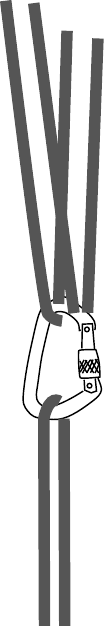
\includegraphics[width=0.65in]{ch04/figs/anchor-2}\end{column}

    \begin{column}{.8\textwidth}

    This figure shows the simplest case, where the angle $A$ has been closed up completely like a pair of
    scissors. $A=0$.
      Suppose that the climber is hanging her weight from this anchor, and her weight amounts to 1000 newtons.
      (A newton is the metric unit of force, equal to about a fifth of a pound.) The vector sum of the upward
      forces from the two ropes on top has to cancel out the downward force of her weight. How much stress is
      placed on each anchor? Verify that the result of vector addition agrees with the result that you would
      have gotten based on arithmetic and common sense.

    \end{column}
  \end{mycolumns}

\end{frame}

\begin{frame}{Galilean vectors}


  \begin{mycolumns}

    \begin{column}{.4\textwidth}\includegraphics[width=4in]{ch04/figs/anchor-3}\end{column}

    \begin{column}{.6\textwidth}

      \newcommand{\degunit}{\ensuremath{\mspace{0mu}^\circ}}

      This example, with $A=120\degunit$, is also especially simple, because the three forces are now
      arranged symmetrically around a circle. Again, the climber's weight is 1000 newtons. What is the
      stress on each anchor?

    \end{column}
  \end{mycolumns}

\end{frame}

\begin{frame}{Relativistic vectors}

\dq
Compare the magnitudes of the relativistic vectors.

  \begin{mycolumns}

    \begin{column}{.4\textwidth}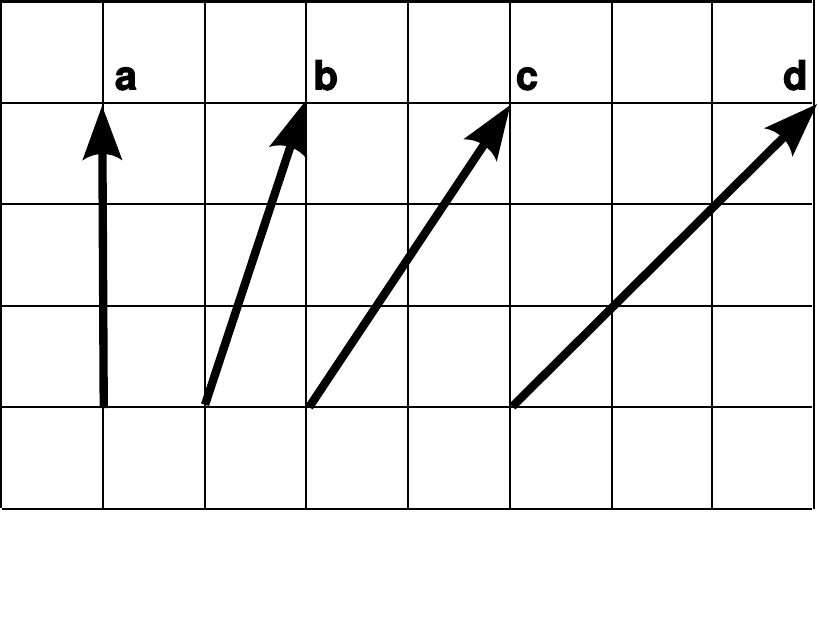
\includegraphics[width=4in]{ch04/figs/leaning-vectors}\end{column}

    \begin{column}{.6\textwidth}

    \end{column}
  \end{mycolumns}

\end{frame}

\begin{frame}{Vectors with the same magnitude}

\dq
The figure shows relativistic vectors on a standard spacetime diagram (time versus position).

  \begin{mycolumns}

    \begin{column}{.4\textwidth}\includegraphics[width=4in]{ch04/figs/congruent-four-vectors}\end{column}

    \begin{column}{.6\textwidth}

Which of these vectors look like they could have the same magnitude as each other, and
which are definitely different? In which case would it be necessary to carry out a Lorentz
transformation in order to be sure?


    \end{column}
  \end{mycolumns}


\end{frame}
